\subsection{Ртутная лампа}
Построим график $d_i^2 = F(i)$ для зелёной линии ртути, приняв 
длину её волны $\lambda (Hg) = 5461$ \AA. По наклону 
полученной прямой рассчитаем базу $L$ интерферометра, используя 
формулу 
\begin{equation}\label{eq::A_2}
  \frac{\lambda}{L} = \frac{1}{4f^2} \frac{\Delta(d_i)}{\Delta(i)}
\end{equation}


\import{./}{hg_green_circ.tex}
По полученным данным построим график:

\begin{figure}[h]
  \center{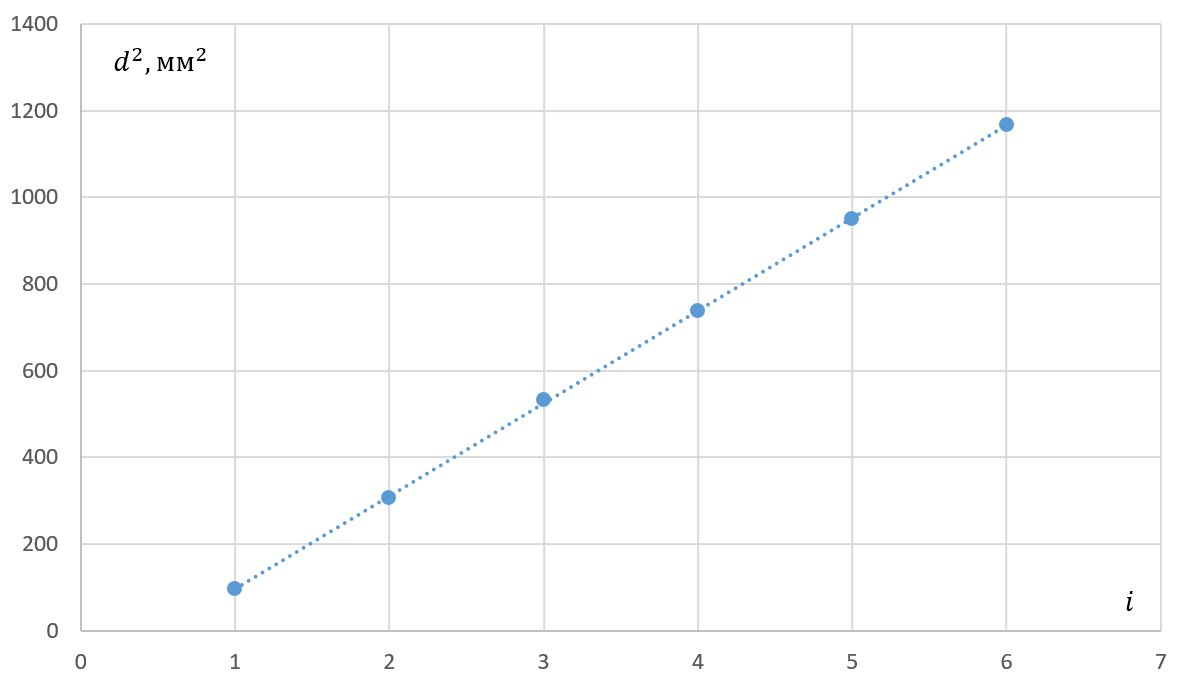
\includegraphics[width=0.7\linewidth]{graph_hg_d_from_i.png}}
\end{figure}

\subsection{Натриевая лампа}